
\documentclass[12pt,a4paper]{article}
\usepackage{fontspec}
\defaultfontfeatures{Ligatures=TeX,Scale=MatchLowercase}
\IfFontExistsTF{Alice-Regular}{
  \setmainfont{Alice-Regular}[
      BoldFont = Alice-Regular,
      ItalicFont = Alice-Regular,
      BoldItalicFont = Alice-Regular,
      BoldFeatures = {FakeBold=1.6},
      ItalicFeatures = {FakeSlant=0.2},
      BoldItalicFeatures = {FakeBold=1.6,FakeSlant=0.2}
  ]
}{
  \setmainfont{Noto Serif}
}
\IfFontExistsTF{Noto Sans}{\setsansfont{Noto Sans}}{}
\usepackage{polyglossia}
\setmainlanguage{russian}
\usepackage[a4paper,left=20mm,right=20mm,top=20mm,bottom=20mm]{geometry}
\usepackage{graphicx}
\usepackage{amsmath,amssymb,amsthm}
\usepackage{booktabs,longtable,tabularx,array,float,multirow}
\usepackage{tikz}
\usepackage[europeanresistors]{circuitikz}
\usepackage{pgfplots}
\usepackage{xcolor}
\usepackage{caption}
\usepackage{fancyhdr}
\usepackage{enumitem}
\pgfplotsset{compat=1.18}
\pagestyle{fancy}
\setlength{\headheight}{15pt}
\fancyhf{}
\renewcommand{\headrulewidth}{0.4pt}
\renewcommand{\footrulewidth}{0.4pt}
\fancyfoot[C]{\thepage}
\newcolumntype{C}{>{\centering\arraybackslash}X}
\renewcommand{\arraystretch}{1.25}

\newcommand{\TitlePage}[2]{
\title{
	МИНОБРНАУКИ РОССИИ

	федеральное государственное автономное образовательное учреждение

	высшего образования

	«Национальный исследовательский университет

	«Московский институт электронной техники»
	\vspace{2em}
}
\author{}
\date{}
\maketitle
\thispagestyle{fancy}
\begin{center}
\Large Отчёт по лабораторной работе №#1\\
по дисциплине «Электротехника»\\
«#2»
\end{center}
\begin{center}
\Large Вариант 2
\end{center}
\vspace{12em}
\begin{table}[H]
\noindent
\begin{tabular*}{\textwidth}{@{\extracolsep{\fill}} p{0.48\textwidth} p{0.52\textwidth}}
Студент & Анисимов А.\,С., ЭН-$25$ \\
[0.5em] Руководитель & Самохин Д.\,В.
\end{tabular*}
\end{table}
\cfoot{Москва 2026}
\pagebreak
\fancyhead[L]{#2}
\fancyhead[R]{Электротехника}
}

\begin{document}
\TitlePage{3}{Исследование резонансных цепей}

\section*{Цель работы}
Исследовать последовательный резонансный контур, определить его основные параметры, построить частотные характеристики и проанализировать поведение напряжений на элементах $R$, $L$ и $C$.

\section*{Исходные данные}
По условию варианта:
\[
L = 23\,\text{мГн}, \qquad C = 0.0075\,\mu\text{Ф} = 7.5\,\text{нФ}, \qquad R = 1200\,\Omega.
\]
Для численных расчётов принято действующее значение источника $E=1\,\text{В}$.

\begin{figure}[H]
\centering
\begin{circuitikz}[american voltages]
\draw
(0,0) to[sV,l=$e(t)$] (0,3)
      to[R,l=$R$] (3,3)
      to[C,l=$C$] (5,3)
      to[L,l=$L$] (5,0)
      -- (0,0);
\draw[->] (2.3,3.35) -- (3.2,3.35) node[midway,above] {$i(t)$};
\end{circuitikz}
\caption{Последовательный резонансный контур.}
\end{figure}

\section*{1. Основные параметры контура}
Волновое сопротивление:
\[
\rho=\sqrt{\frac LC}=\sqrt{\frac{0.023}{7.5\cdot 10^{-9}}}
\approx 1751.190\,\Omega.
\]

Резонансная частота:
\[
F_p=\frac1{2\pi\sqrt{LC}}
=\frac1{2\pi\sqrt{0.023\cdot 7.5\cdot 10^{-9}}}
\approx 12117.850\,\text{Гц}.
\]

Добротность:
\[
Q=\frac{\rho}{R}=\frac{1751.190}{1200}
\approx 1.459.
\]

Относительная полоса пропускания:
\[
d=\frac1Q \approx 0.685.
\]

Частота максимума напряжения на индуктивности:
\[
F_L=\frac{F_p}{\sqrt{1-\frac1{2Q^2}}}
\approx 13852.660\,\text{Гц}.
\]

Частота максимума напряжения на конденсаторе:
\[
F_C=F_p\sqrt{1-\frac1{2Q^2}}
\approx 10600.296\,\text{Гц}.
\]

\section*{2. Формулы для расчёта токов, напряжений и угла сдвига фаз}
Для последовательной цепи:
\[
X_L=\omega L,\qquad X_C=\frac1{\omega C},\qquad
|Z|=\sqrt{R^2+(X_L-X_C)^2}.
\]
Тогда
\[
I=\frac E{|Z|}, \qquad U_R=IR, \qquad U_L=IX_L, \qquad U_C=IX_C,
\]
\[
\varphi = \arctan\frac{X_L-X_C}R.
\]

Эти формулы использованы во всех дальнейших вычислениях. Такой выбор обоснован тем, что в последовательном контуре один и тот же ток проходит через все элементы, а различие режимов определяется только частотной зависимостью реактивных сопротивлений.

\section*{3. Расчётная таблица}
\begin{center}
\small
\begin{tabular}{|c|c|c|c|c|c|c|}
\hline
Частота & $F$, Гц & $I$, мА & $U_R$, В & $U_L$, В & $U_C$, В & $\varphi$, град \\
\hline
$F_p$ & 12117.9 & 0.833 & 1.000 & 1.459 & 1.459 & 0.00 \\ \hline
$0.1F_p$ & 1211.8 & 0.058 & 0.069 & 0.010 & 1.008 & -86.04 \\ \hline
$0.3F_p$ & 3635.4 & 0.184 & 0.220 & 0.096 & 1.072 & -77.27 \\ \hline
$0.5F_p$ & 6058.9 & 0.346 & 0.416 & 0.303 & 1.213 & -65.45 \\ \hline
$0.7F_p$ & 8482.5 & 0.571 & 0.685 & 0.700 & 1.428 & -46.76 \\ \hline
$2F_p$ & 24235.7 & 0.346 & 0.416 & 1.213 & 0.303 & 65.45 \\ \hline
$3F_p$ & 36353.6 & 0.207 & 0.249 & 1.090 & 0.121 & 75.59 \\ \hline
$F_L$ & 13852.7 & 0.776 & 0.931 & 1.553 & 1.189 & 21.39 \\ \hline
$F_C$ & 10600.3 & 0.776 & 0.931 & 1.189 & 1.553 & -21.39 \\ \hline
\end{tabular}
\end{center}

Из таблицы видно:
\begin{itemize}[leftmargin=1.2cm]
\item при $F=F_p$ реактивные сопротивления равны, поэтому $\varphi\approx 0^\circ$, а всё входное напряжение падает на резисторе;
\item при $F<F_p$ цепь носит ёмкостный характер, следовательно $\varphi<0$;
\item при $F>F_p$ цепь носит индуктивный характер, следовательно $\varphi>0$;
\item максимумы $U_L$ и $U_C$ достигаются не ровно в точке резонанса, а на частотах $F_L$ и $F_C$.
\end{itemize}

\section*{4. АЧХ и ФЧХ}
\begin{figure}[H]
\centering
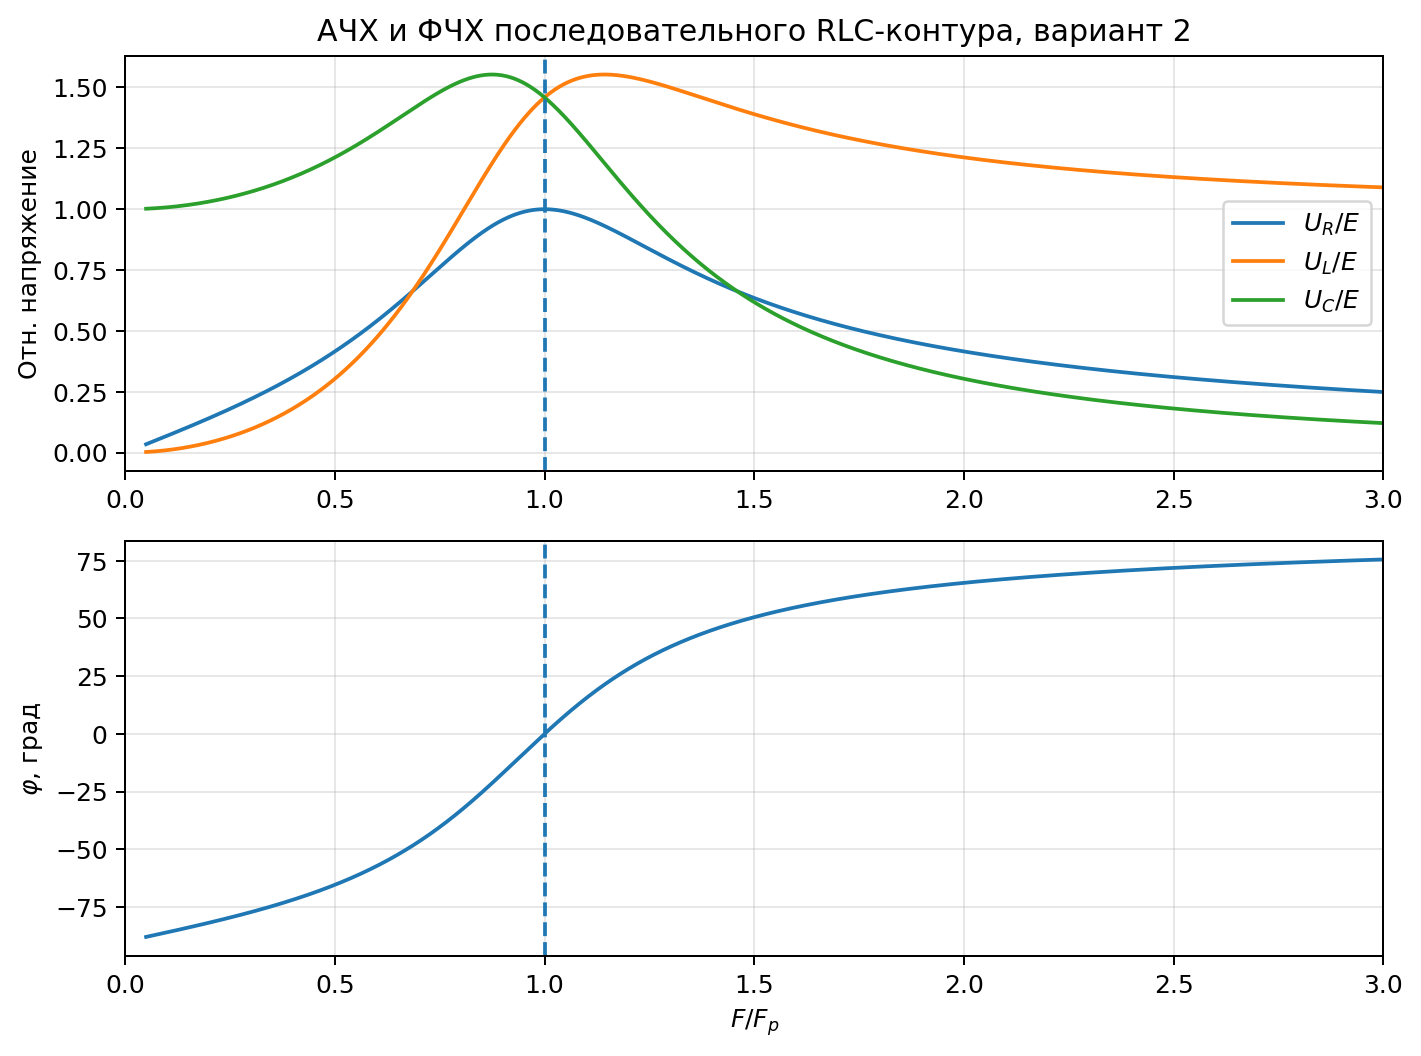
\includegraphics[width=0.92\textwidth]{img/lab3_afh_fch.png}
\caption{Рассчитанные АЧХ и ФЧХ.}
\end{figure}

\section*{5. Векторные диаграммы}
Ниже ток направлен вдоль действительной оси.

\begin{figure}[H]
\centering
\begin{minipage}[t]{0.32\textwidth}
\centering
\begin{tikzpicture}[scale=1.0,>=stealth]
\draw[->] (-0.2,0) -- (3,0) node[right] {Re};
\draw[->] (0,-2.0) -- (0,2.0) node[above] {Im};
\draw[->,thick,blue] (0,0) -- (1.8,0) node[below right] {$U_R$};
\draw[->,thick,red] (1.8,0) -- (1.8,1.4) node[right] {$U_L$};
\draw[->,thick,teal] (1.8,1.4) -- (1.8,0) node[above right] {$U_C$};
\draw[->,ultra thick,purple] (0,0) -- (1.8,0) node[above left] {$E$};
\node at (1.0,-2.0) {$F=F_p$};
\end{tikzpicture}
\end{minipage}
\begin{minipage}[t]{0.32\textwidth}
\centering
\begin{tikzpicture}[scale=1.0,>=stealth]
\draw[->] (-0.2,0) -- (3,0) node[right] {Re};
\draw[->] (0,-2.0) -- (0,2.0) node[above] {Im};
\draw[->,thick,blue] (0,0) -- (1.2,0) node[above right] {$U_R$};
\draw[->,thick,red] (1.2,0) -- (1.2,0.9) node[right] {$U_L$};
\draw[->,thick,teal] (1.2,0.9) -- (1.2,-1.3) node[above right] {$U_C$};
\draw[->,ultra thick,purple] (0,0) -- (1.2,-1.3) node[below] {$E$};
\node at (1.0,-2.0) {$F=0.5F_p$};
\end{tikzpicture}
\end{minipage}
\begin{minipage}[t]{0.32\textwidth}
\centering
\begin{tikzpicture}[scale=1.0,>=stealth]
\draw[->] (-0.2,0) -- (3,0) node[right] {Re};
\draw[->] (0,-2.0) -- (0,2.0) node[above] {Im};
\draw[->,thick,blue] (0,0) -- (1.2,0) node[below] {$U_R$};
\draw[->,thick,red] (1.2,0) -- (1.2,2.2) node[right] {$U_L$};
\draw[->,thick,teal] (1.2,2.2) -- (1.2,1.3) node[below right] {$U_C$};
\draw[->,ultra thick,purple] (0,0) -- (1.2,1.3) node[above right] {$E$};
\node at (1.0,-2.0) {$F=2F_p$};
\end{tikzpicture}
\end{minipage}
\caption{Качественные векторные диаграммы для трёх характерных частот.}
\end{figure}

\section*{Вывод}
Полностью рассчитан последовательный резонансный контур. Найдены волновое сопротивление 
$\rho\approx 1751.2\,\Omega$, резонансная частота $F_p\approx 12117.9\,\text{Гц}$, 
добротность $Q\approx 1.459$ и относительная полоса пропускания $d\approx 0.685$. 
Составлена таблица значений тока, напряжений и фазового угла для заданного набора 
частот, а также построены частотные характеристики. Расчёты показывают, что вблизи 
резонанса напряжения на реактивных элементах превышают входное напряжение, что и 
является характерным признаком резонансного режима.

\end{document}
